\newpage
\section{Поиск парковочного места}

Поиск парковочного места осуществляется по тому же принципу, что и в реальной жизни: робот-машинка двигается параллельно припаркованному ряду автомобилей с постоянной скоростью $v$, одновременно сканируя пространство справа от себя. Сканирование олицетворяет собой измерение расстояния между роботом и объектами справа от него.
Измерения ($S_{front}$ и $S_{rear}$) производятся двумя ультразвуковыми дальномерами, расположение которых на роботе изображено на рисунке~\ref{robot_and_us_sensors}.

% Важно! Передний датчик покрасить в красный, задний в синий!
\begin{figure}[h!]
	\begin{minipage}[h]{0.47\textwidth}
		\centering{ 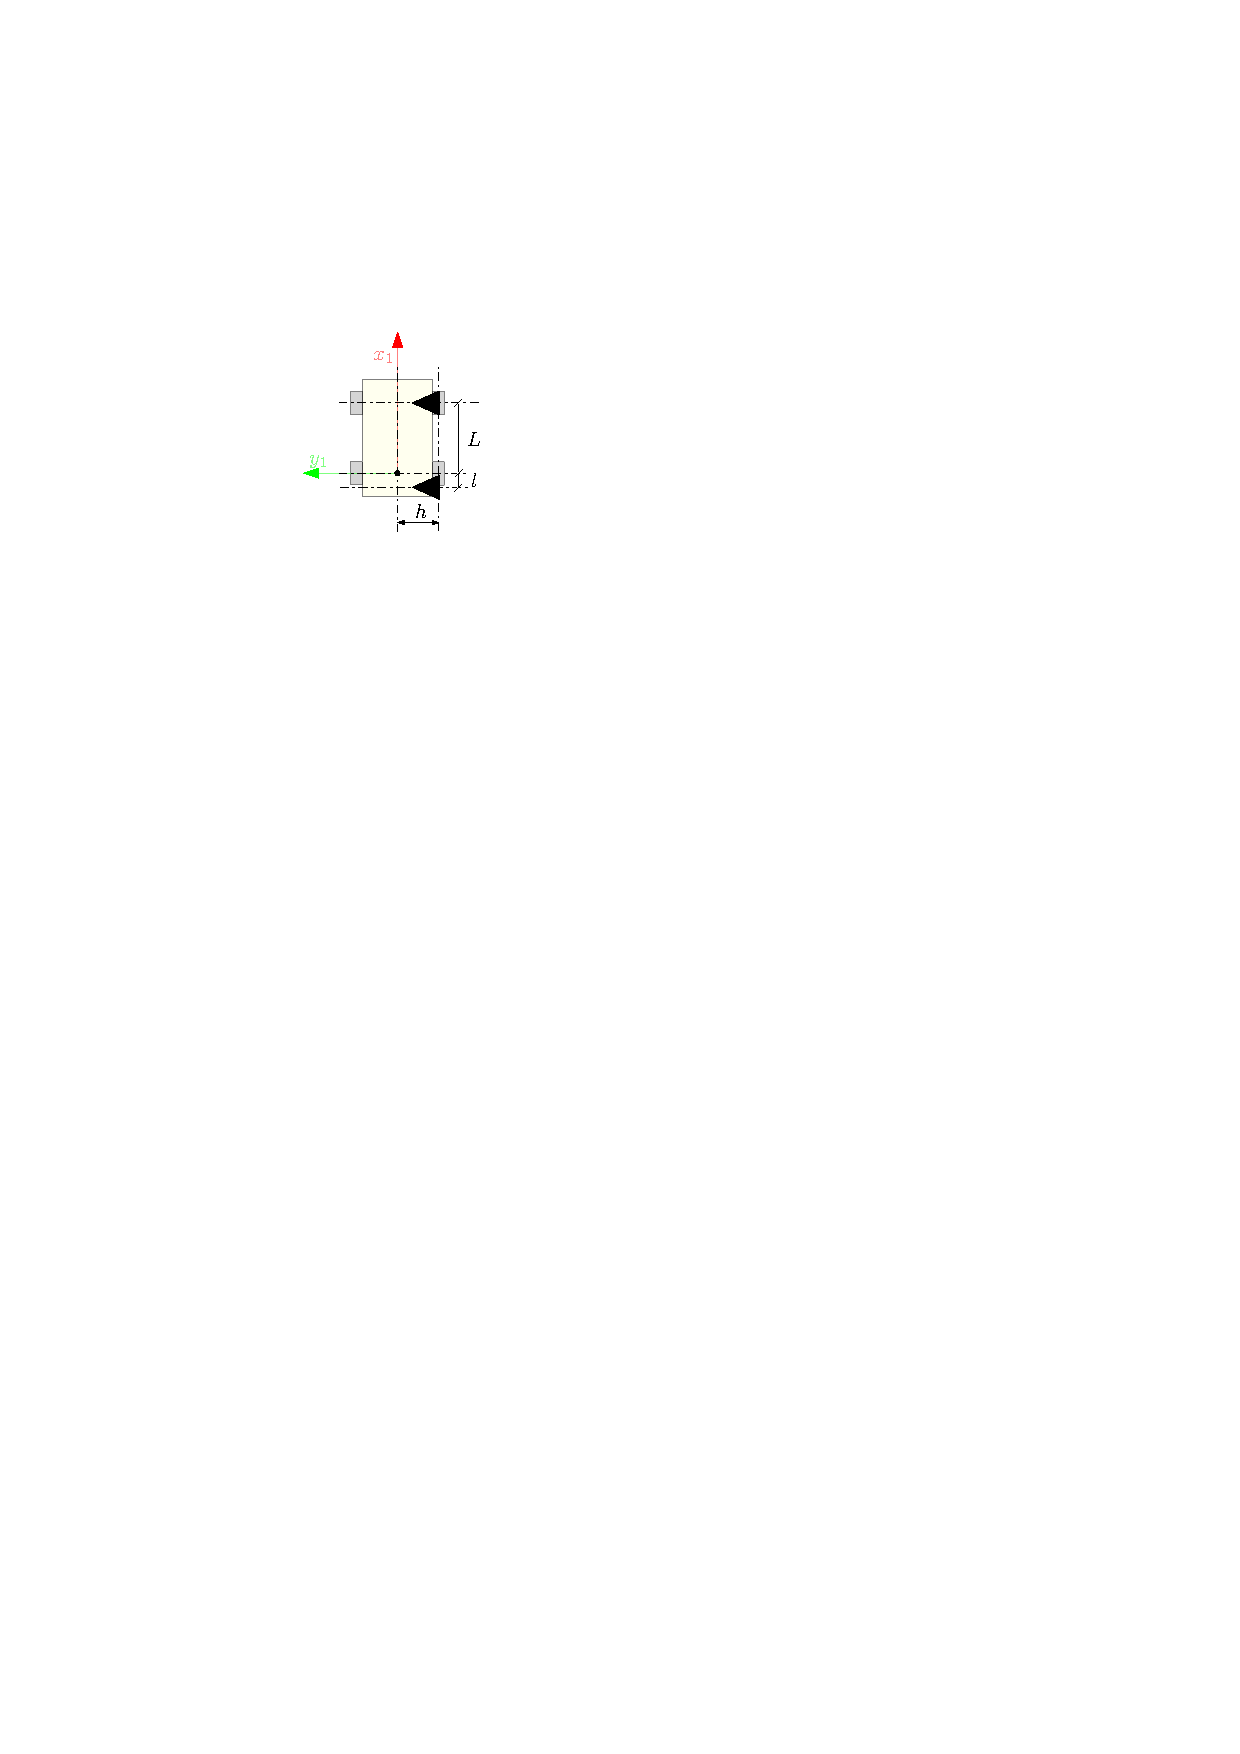
\includegraphics[width=0.7\textwidth]{robot_sensors_schema_top.pdf} \\ a) вид сверху}
	\end{minipage}
	\hfill
	\begin{minipage}[h]{0.47\textwidth}
		\centering{ 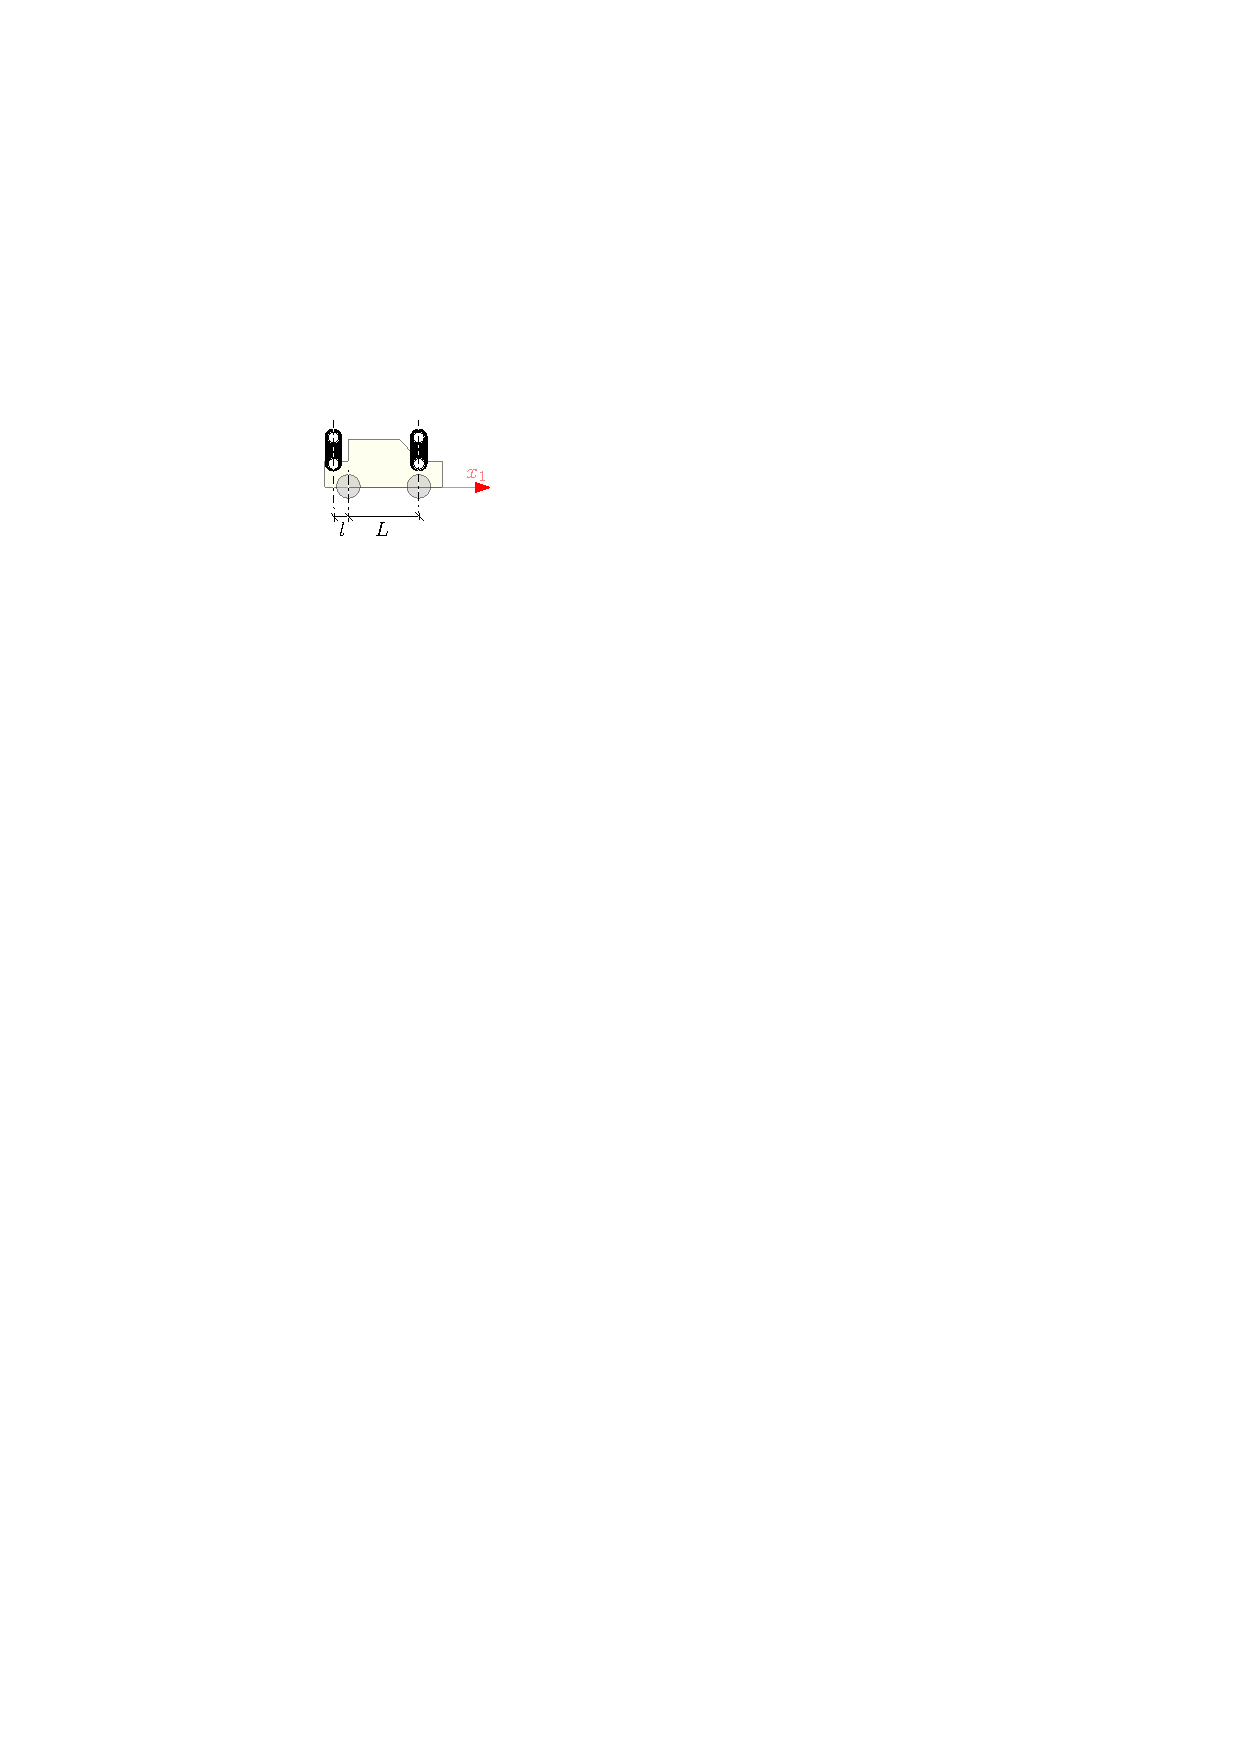
\includegraphics[width=0.9\textwidth]{robot_sensors_schema_right.pdf} \\ б) вид справа (по ходу движения)}
	\end{minipage}
	\caption{Расположение ультразвуковых дальномеров.}
	\label{robot_and_us_sensors}
\end{figure}

Измерения показаний ультразвуковых дальномеров представляются в локальной СК робота точками ($p_{1}$ и $p_{2}$)~\eqref{us_points}. После чего преобразуются в глобальную СК путем перемножения матрицы однородных преобразования $H$ и соответствующей измеренной точки~\eqref{}--\eqref{label}

\begin{equation}\label{us_points}
p_{1} = 
\begin{bmatrix}
x_{p_1} \\
y_{p_1} \\
\end{bmatrix}
=
\begin{bmatrix}
L \\
- (S_{front} + d) \\
\end{bmatrix}\!\!;~
p_{2} = 
\begin{bmatrix}
x_{p_2} \\
y_{p_2} \\
\end{bmatrix}
=
\begin{bmatrix}
-l \\
- (S_{rear} + d) \\
\end{bmatrix}\!\!.
\end{equation}
где $l$~--- расстояние между задней осью и ультразвуковым дальномером, закрепленным на задней части робота; $d$~--- расстояние от продольной оси робота до сенсоров дальномеров.

\begin{equation}
	H = 
	\begin{bmatrix}
		\cos{\theta} & -\sin{\theta} & 0 & x \\
		\sin{\theta} & \cos{\theta} & 0 & y \\
		0 & 0 & 1 & 0\\
		0 & 0 & 0 & 1
	\end{bmatrix}
\end{equation}

\begin{equation}
	P = H \cdot p = 
	\begin{bmatrix}
		x_P\\ y_P\\0\\1
	\end{bmatrix}
	= 
	\begin{bmatrix}
		\cos{\theta} & -\sin{\theta} & 0 & x \\
		\sin{\theta} & \cos{\theta} & 0 & y \\
		0 & 0 & 1 & 0\\
		0 & 0 & 0 & 1
	\end{bmatrix} 
	\cdot
	\begin{bmatrix}
		x_p \\ y_p \\ 0\\ 1
	\end{bmatrix}
\end{equation}

В результате описанного выше сканирования строится карта. Построение карты происходит в несколько этапов:

\begin{enumerate}
	\item робот движется вдоль припаркованного ряда автомобилей на расстоянии от него не более, чем 0.3 метра;
	\item записываются измерения расстояний с дальномеров не более, чем 0.5 метров;
	\item из массива данных с картой удаляются все точки дальше, чем среднее арифметическое расстояний.
\end{enumerate}


В результате этой процедуры на карте остаются проекции препятствий на плоскость дорожного полотна. На рисунке~\ref{map_real} показана зона проведения эксперимента, на рисунке~\ref{map} -- пример полученной карты.\footnote{Представленные на рисунке~\ref{map} результаты фильтрации сканированных данных с дальномеров были получены не в том же эксперименте, что на рисунках~\ref{map_real} и \ref{parking_place}}

После готовности карты, на ней разыскивается парковочное место подходящего размера, который задается постоянным параметром. При чем, линия параллельно которой будет парковаться робот выбирается как среднее от отфильтрованных данных карты. На нашей карте такое место определяется поиском двух соседних точек таких, что расстояние между ними вдоль линии движения робота должно быть больше постоянного параметра, о котором говорилось выше. Пример карты с выделенным парковочным местом показан на рисунке~\ref{parking_place}.

\begin{figure}[h]
	\centering
	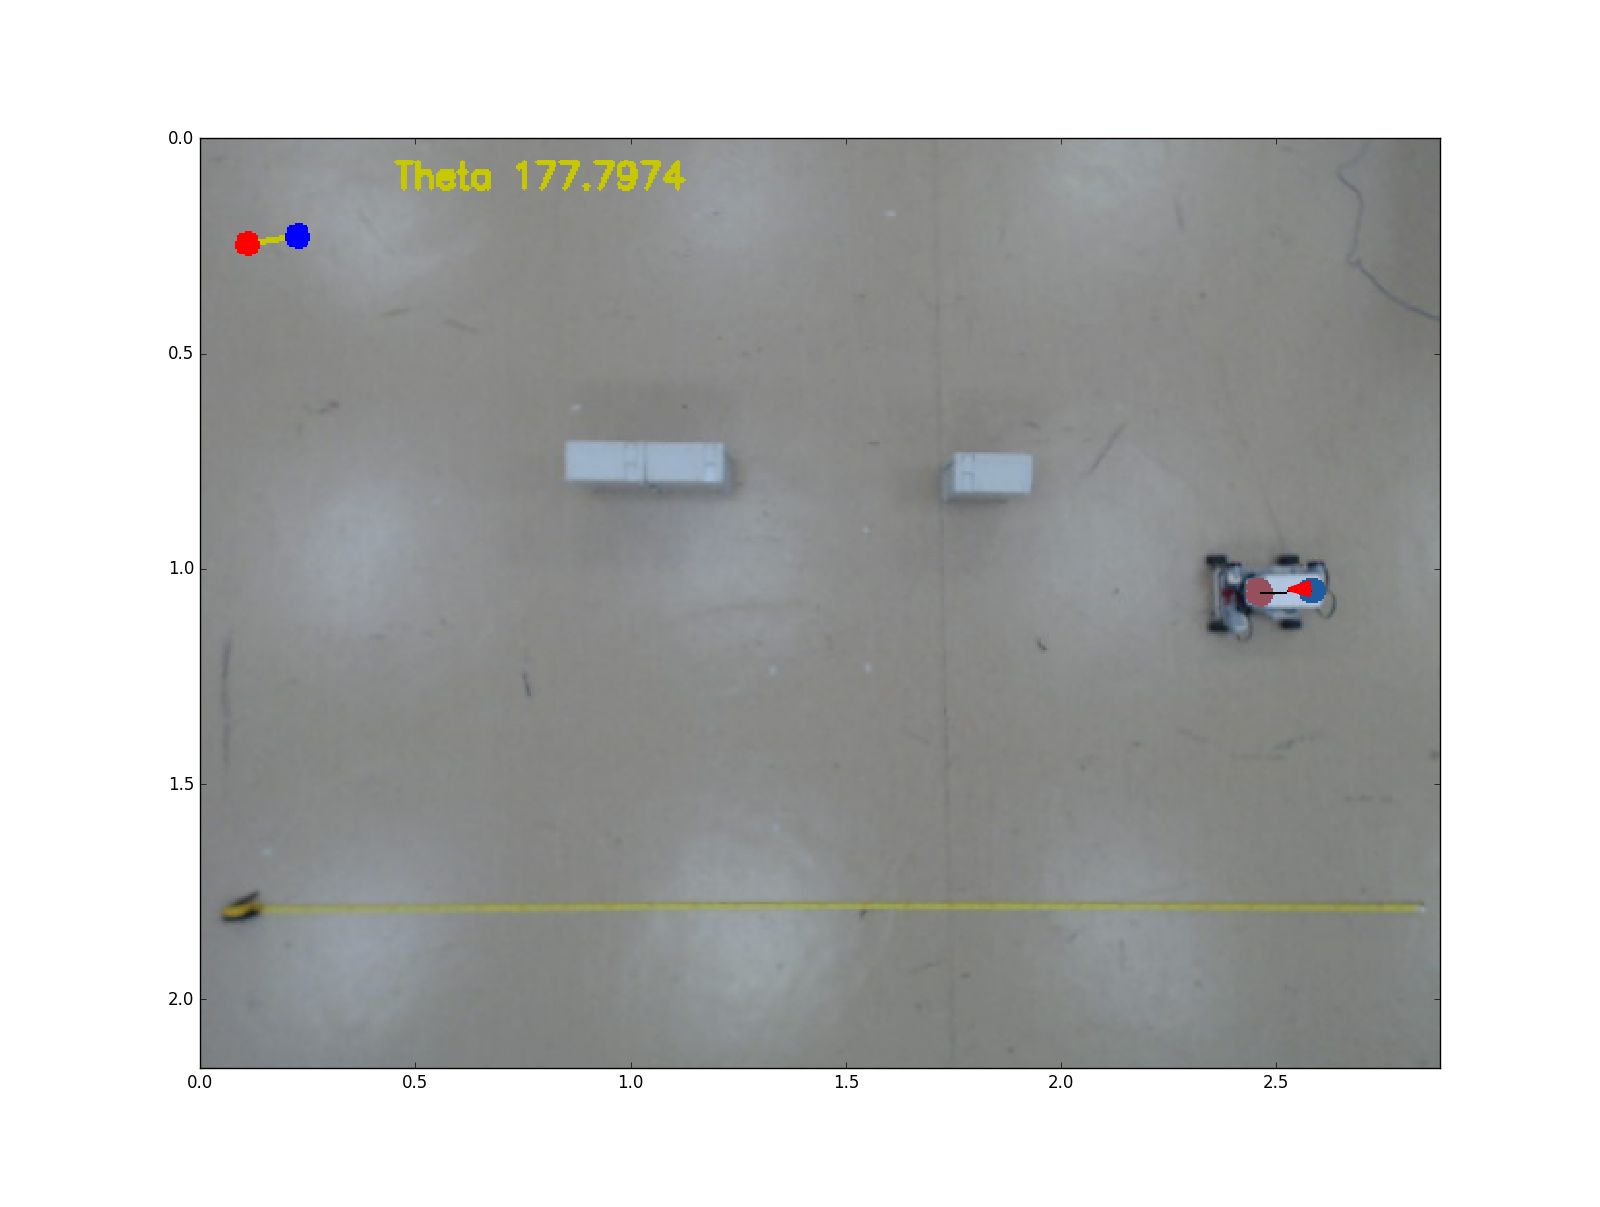
\includegraphics[width=\textwidth]{map_real.png}
	\caption{Зона проведения эксперимента в реальности. Вид сверху.}
	\label{map_real}
\end{figure}

\begin{figure}[h!]
	\centering{ 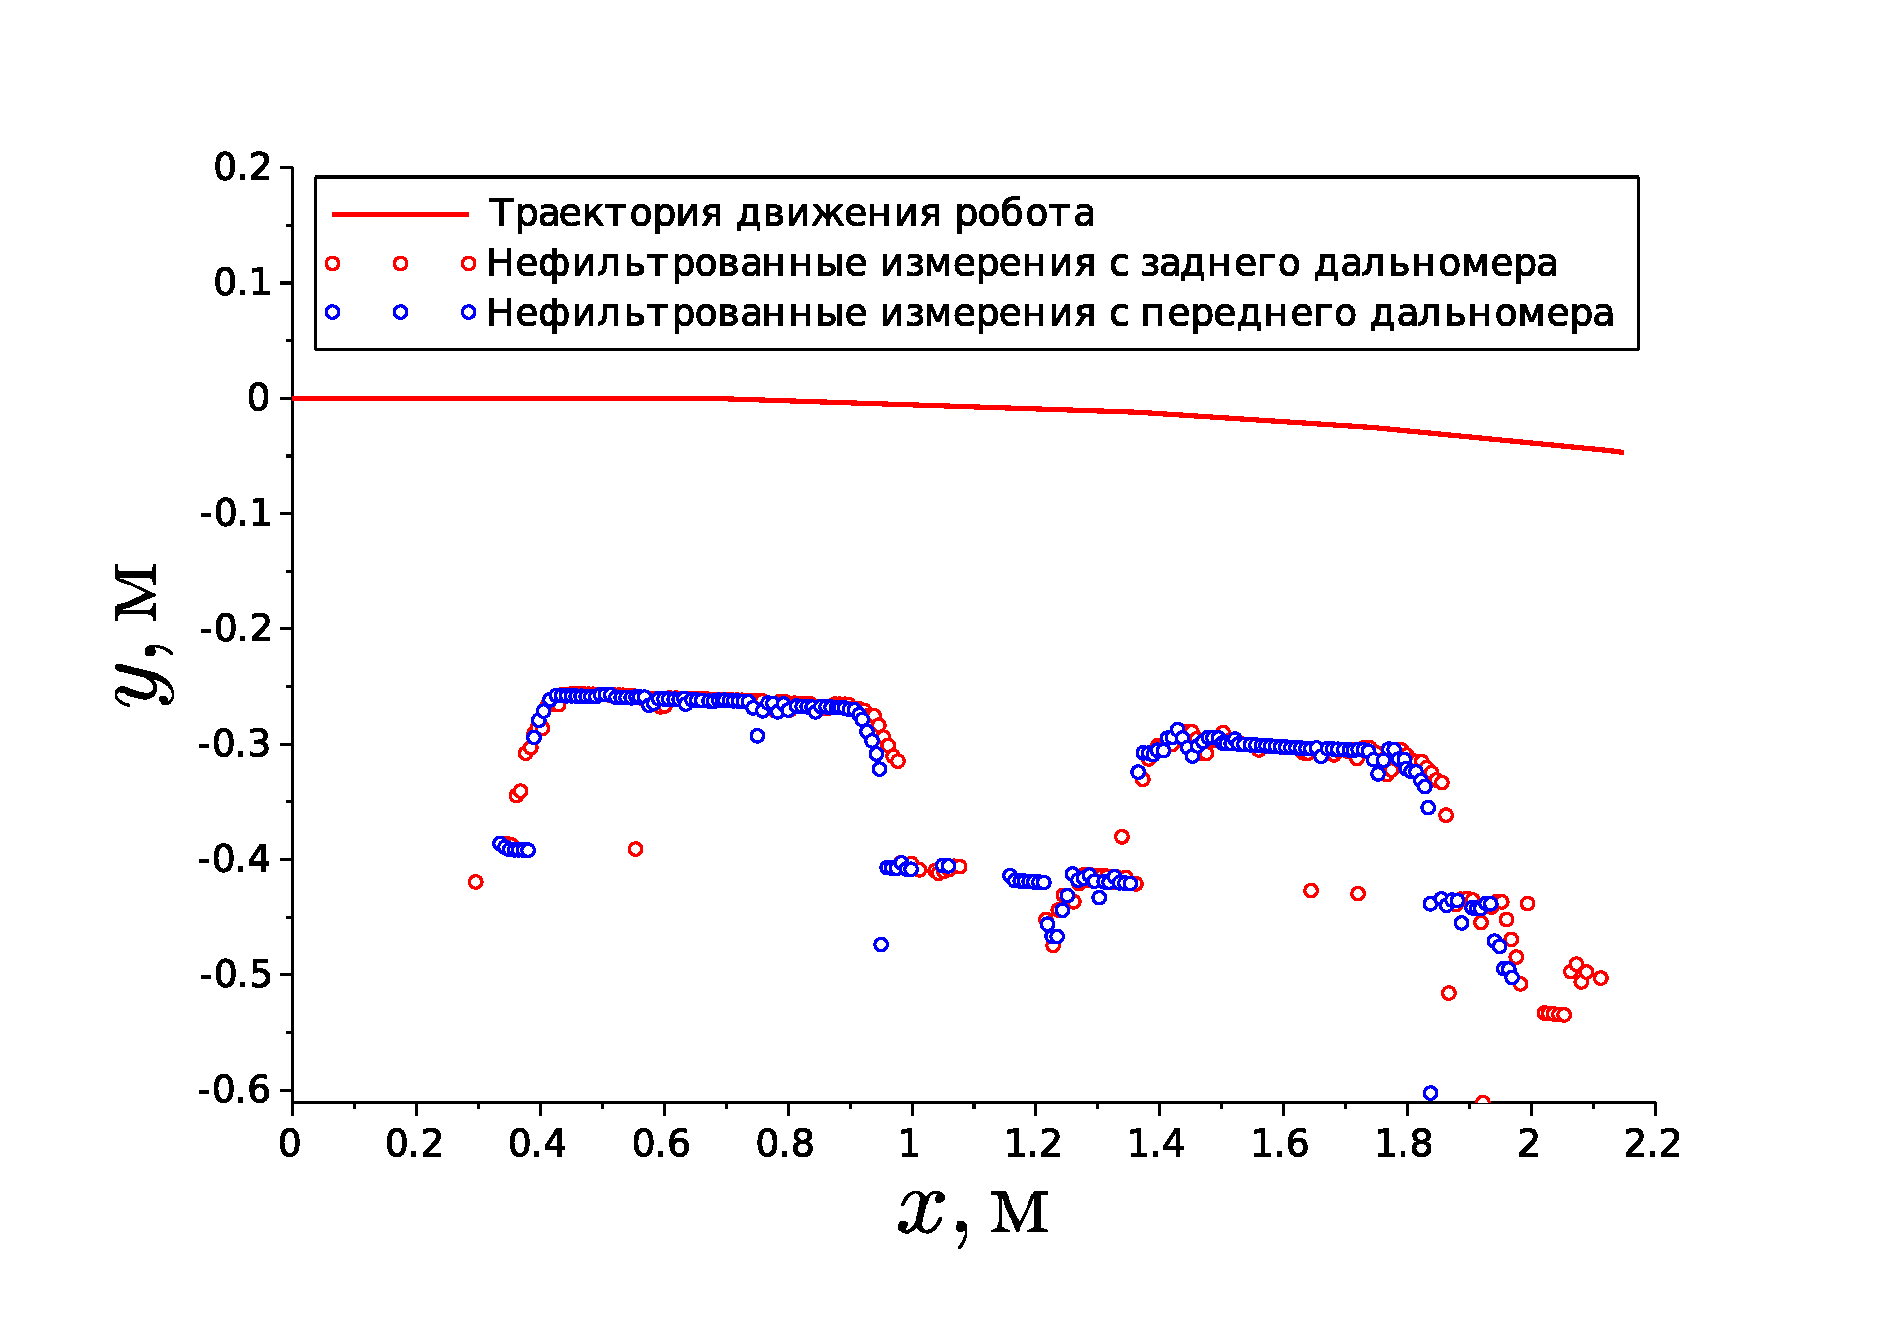
\includegraphics[width=0.9\textwidth]{_map_no_filtred.pdf} \\ a) \\}
	\centering{ 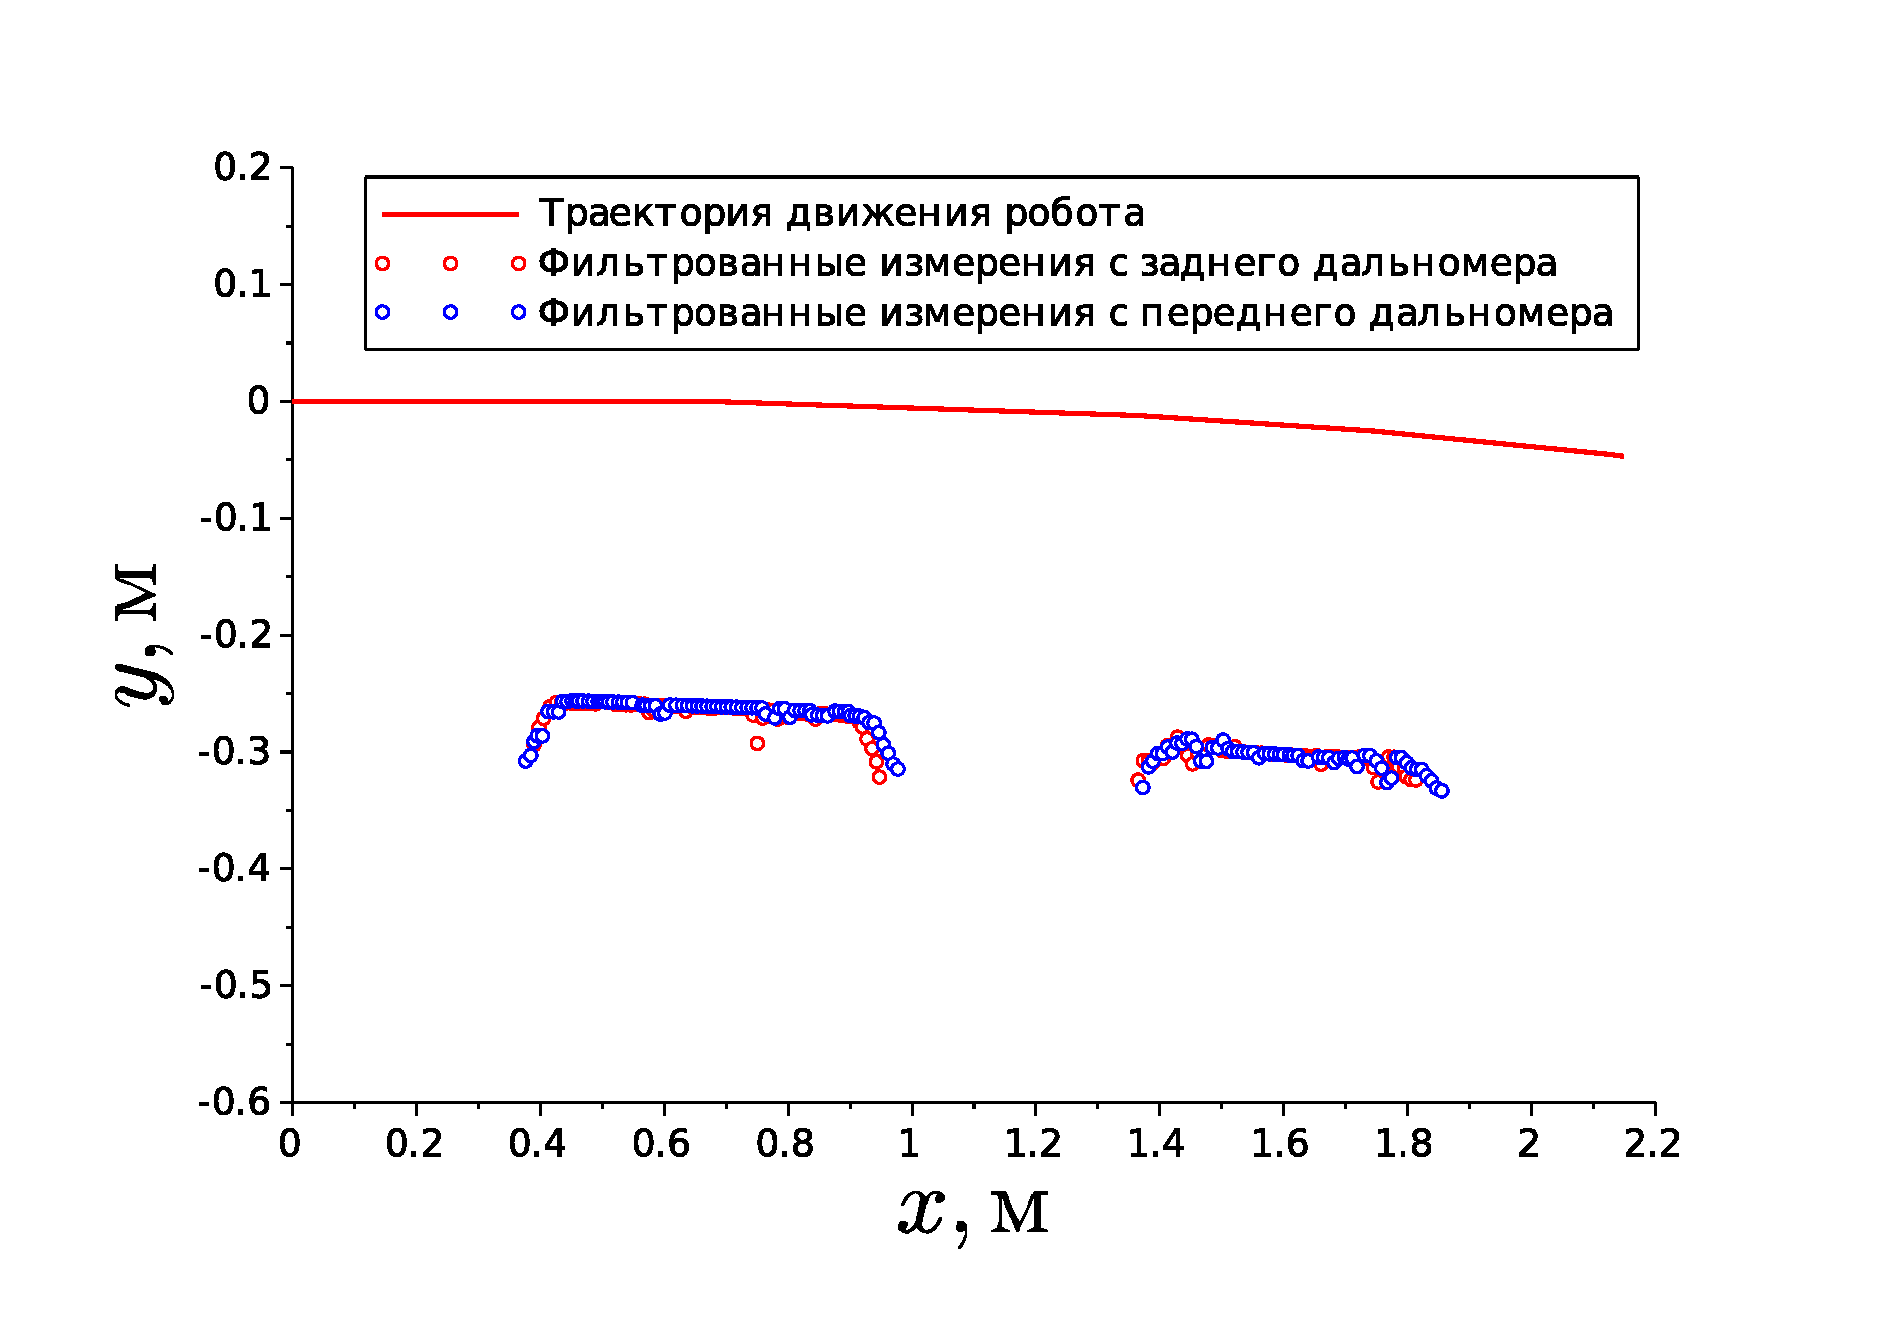
\includegraphics[width=0.9\textwidth]{_map_filtred.pdf} \\ б) }
	\caption{Результаты сканирования: a~--- карта до фильтрации, б~--- карта после фильтрации.}
	\label{map}
\end{figure}

\begin{figure}[h]
	\centering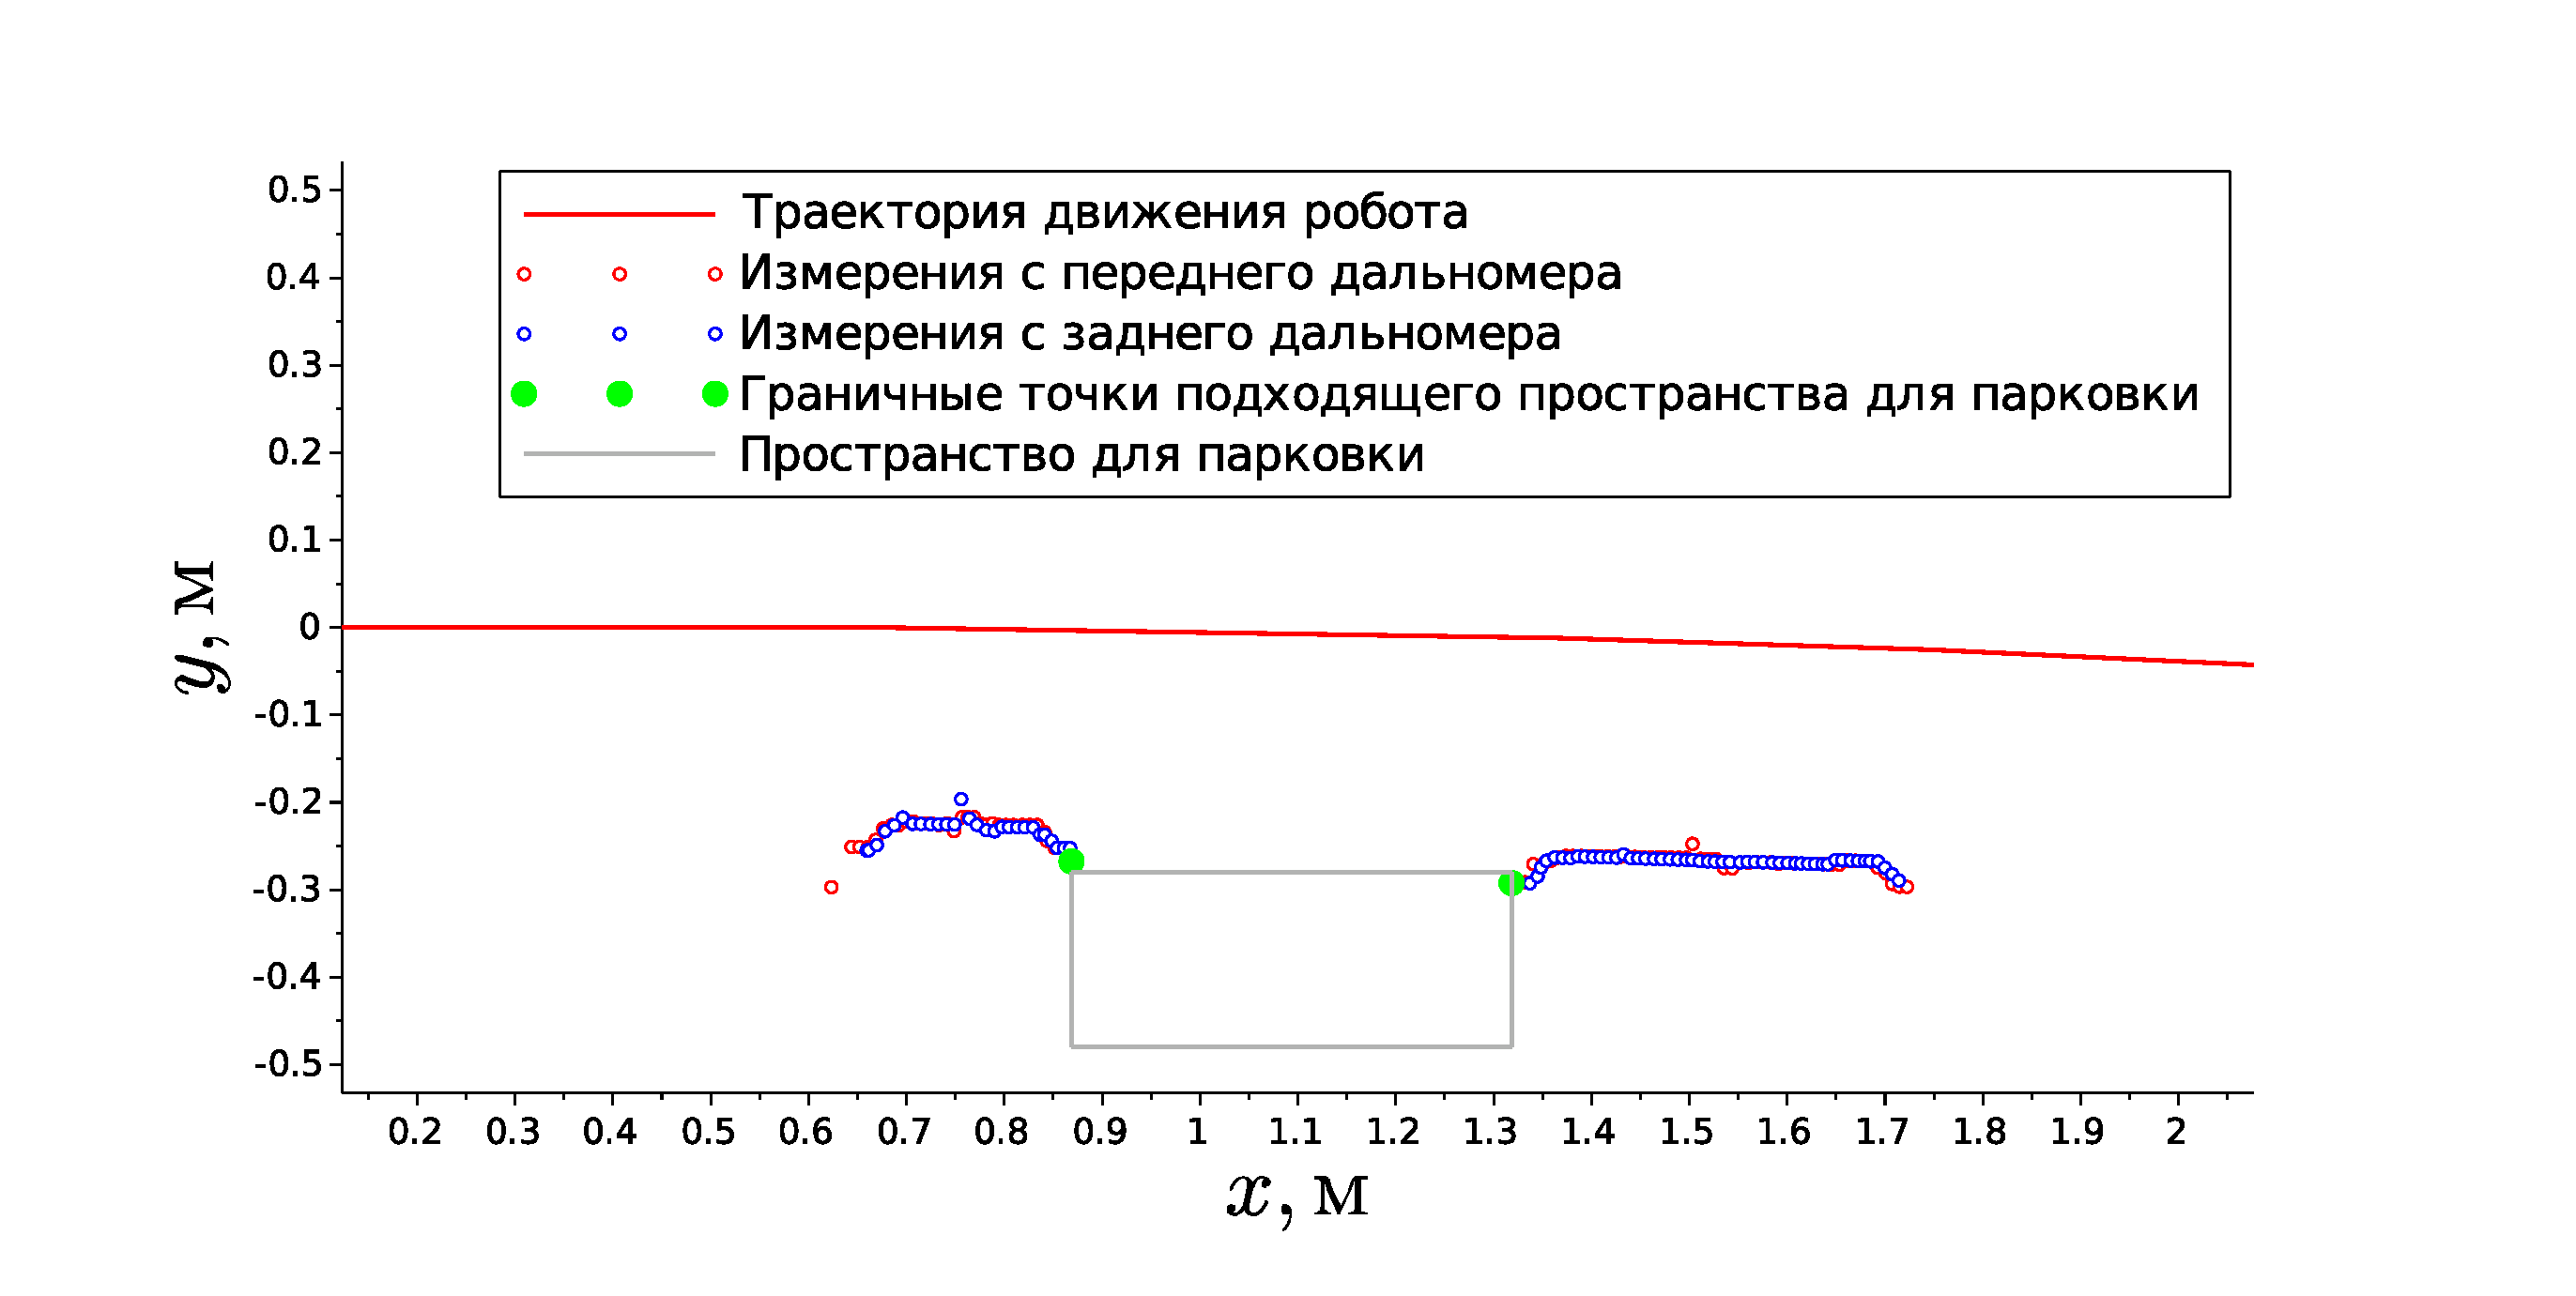
\includegraphics[width=\textwidth]{parking_place.pdf}
	\caption{Карта с выделенным парковочным местом.}
	\label{parking_place}
\end{figure}

\clearpage

